\def\pgfsysdriver{pgfsys-dvipdfm.def}
%\documentclass[aspectratio=1610]{beamer}
\documentclass{beamer}
\usetheme[progressbar=head, titleformat=allcaps,block=fill]{metropolis}
\usepackage[orientation=landscape,size=custom,width=16,height=11.15,scale=.5,debug]{beamerposter}

%%% PACKAGES AND INPUTS
\usepackage{pgfopts}
\usepackage{pgfpages}
\usepackage{graphicx}
\usepackage{xcolor}
\usepackage{tikz}
\usetikzlibrary{3d,hyperref}
\usepackage{verbatim}
\usepackage{comment}
%\input{153controls}
\usepackage{pgfplots}
\usepackage{linalgjh}

\usepackage{multicol}


%%% POLAR SETUP
\usepgfplotslibrary{polar}
\pgfplotsset{compat=1.10}
\pgfplotsset{mypolarplot/.style={%
  clip=false, % needed for double line (last \addplot command)
  domain=0:360, % plot full cycle
  samples=180, % number of samples; can be locally adjusted
  grid=both, % display major and minor grids
  major grid style={black}, 
  minor x tick num=3, % 3 minor x ticks between majors
  minor y tick num=1, % 1 minor y tick between majors
  xtick={0,45,...,359},
  xticklabels={%
    $0$,
    $\frac{ \pi}{4}$,
    $\frac{ \pi}{2}$,
    $\frac{3\pi}{4}$,
    $\pi$,
    $\frac{5\pi}{4}$,
    $\frac{3\pi}{2}$,
    $\frac{7\pi}{4}$
  },
  yticklabel style={anchor=north}, % move label position
}}

%%%% COLORS
\definecolor{gold}{HTML}{ffb81c}
\definecolor{heypurple}{HTML}{6B0FFF}
\definecolor{darkgold}{HTML}{5A440D}
\definecolor{darkblue}{HTML}{00268D}
\definecolor{proof}{RGB}{55,54,172}
\definecolor{nicegreen}{RGB}{0,127,35}
\definecolor{remgrey}{RGB}{179,179,179}
\definecolor{Purple}{HTML}{3C0940}
\definecolor{darkgreen}{HTML}{214009}
\definecolor{Orange}{HTML}{7F2000}
\definecolor{Blue}{HTML}{003E78}
\definecolor{Gold}{HTML}{FFCB0A}
\definecolor{gvsublue1}{HTML}{0065a4}
\definecolor{gvsublue2}{HTML}{88B3DA}
\definecolor{unlred}{HTML}{D00000}
\definecolor{DordtGrey}{RGB}{127,127,127}
\definecolor{newred}{HTML}{85140D}
\definecolor{msugreen}{HTML}{023328}
\definecolor{seafoam}{HTML}{127F67}
\definecolor{mnmaroon}{HTML}{790018}
\definecolor{mngold}{HTML}{FFD75F}
\definecolor{fallfoliage}{HTML}{763626}
\definecolor{stone}{HTML}{336B87}
\definecolor{shadow}{HTML}{2A3132}
\definecolor{grass}{HTML}{486B00}
\definecolor{thundercloud}{HTML}{505160}
\definecolor{meadow}{HTML}{598234}
\definecolor{ink}{HTML}{20232A}
\definecolor{rubyred}{HTML}{A01D26}
\definecolor{stormysea}{HTML}{335252}
\definecolor{rust}{HTML}{AA4B41}
\definecolor{forest}{HTML}{1E434C}
\definecolor{crimson}{HTML}{8D230F}
\definecolor{vtgold}{HTML}{C99E10}
\definecolor{vtrust}{HTML}{9B4F0F}

%%%% BEAMER THEMES AND OPTIONS
%\usetheme[progressbar=head,block=fill]{metropolis}
%\setbeameroption{show notes on second screen}
%\metroset{titleformat=smallcaps,block=transparent}
%\usecolortheme{owl}
\setbeamercolor{progress bar}{fg=heypurple,bg=heypurple!30}
\setsansfont[BoldFont={Graphik Semibold},Numbers={Produkt}]{Graphik}


%%% Dordt
%\setbeamercolor{alerted text}{fg=gold}
%\setbeamercolor{normal text}{fg=black}
%%%\setbeamercolor{block}{transparent}
%%%\setbeamercolor{sectionpage}{bg=white}
%%%\setbeamercolor{titleformatpage}{bg=white}
%\setbeamercolor{frametitle}{fg=gold,bg=black!2}
%%%%% GREEN OPTION
%%%\setbeamercolor{alerted text}{fg=seafoam} 
%%%\setbeamercolor{frametitle}{bg=msugreen}



%%% Purple
\setbeamercolor{alerted text}{fg=heypurple}
\setbeamercolor{normal text}{fg=black}
%%\setbeamercolor{block}{transparent}
%%\setbeamercolor{sectionpage}{bg=white}
%%\setbeamercolor{titleformatpage}{bg=white}
\setbeamercolor{frametitle}{fg=heypurple,bg=black!2}
%%%% GREEN OPTION
%%\setbeamercolor{alerted text}{fg=seafoam} 
%%\setbeamercolor{frametitle}{bg=msugreen}

%%% UMICH OPTION
%\setbeamercolor{alerted text}{fg=gold}
%\setbeamercolor{frametitle}{bg=Blue}

%%% MN OPTION
%\setbeamercolor{alerted text}{fg=gold}
%\setbeamercolor{frametitle}{bg=mnmaroon}

%%% FALL MOUNTAIN
%\setbeamercolor{alerted text}{fg=fallfoliage}
%\setbeamercolor{frametitle}{bg=shadow}
%\setbeamercolor{alerted text}{fg=stone}
%\setbeamercolor{alerted text}{fg=grass}

%%% ICELAND
%\setbeamercolor{alerted text}{fg=meadow}
%\setbeamercolor{frametitle}{bg=thundercloud}


%%% VERMONT
%\setbeamercolor{alerted text}{fg=crimson}
%\setbeamercolor{alerted text}{fg=vtrust}
%\setbeamercolor{frametitle}{bg=thundercloud}


%%% INDUSTRIAL
%\setbeamercolor{alerted text}{fg=rubyred}
%\setbeamercolor{frametitle}{bg=ink}

%%% SAN FRANCISCO
%\setbeamercolor{alerted text}{fg=rust}
%\setbeamercolor{frametitle}{bg=stormysea}


%%%% MACROS
\def\rem#1{{\hfill \textit{\tiny {\color{remgrey} {#1}}}}}
\def\h#1{\alert{#1}}
\def\C{{\mathbb C}}
\def\Z{{\mathbb Z}}
\def\F{{\mathbb F}}
\def\bF{{\mathbb F}}
\def\Q{{\mathbb Q}}
\def\R{{\mathbb R}}
\def\P{{\mathbb P}}
\def\A{{\mathbb A}}
\def\N{{\mathbb N}}
\def\i{\mathbf i}}
\def\j{\mathbf j}}
\def\k{\mathbf k}}
\def\proj{{\text{proj}}}
\def\comp{{\text{comp}}}
\def\set#1{\left\{ {#1} \right\}}
\def\setof#1#2{{\left\{#1\,:\,#2\right\}}}


%%%% ENVIRONMENTS
\newenvironment{proof-idea}{\noindent{\alert{Proof Idea.}}\hspace*{1em}}{\qed\bigskip\\}
\newtheorem{conj}{Conjecture}
\newtheorem{prop}{Proposition}
\newtheorem{cor}{Corollary}
\newtheorem{defn}{Definition}
\newtheorem{question}{Question}
\newtheorem{goal}{Goal}

\usepackage{cancel}
\newcommand\lheq{\mathrel{\overset{\makebox[0pt]{\mbox{\normalfont\tiny\sffamily \alert{L'H}}}}{=}}}

\title{\S 1.2-1.3: Limits and the Derivative at a Point}
%\subtitle{Welcome!}
\author{Dr.\ Mike Janssen}
\date{January 20, 2021}

\begin{document}



\frame{\titlepage}

\frame{
	\frametitle{Preview Activity 1.2.1 Discussion}

}

\frame{
	\frametitle{Why do we need limits?}
	
	\begin{itemize}
	\item Limits give a precise way to talk about trends in function values.
	
	\item They answer the question: what is $f(x)$ (output) doing as $x$ (input) approaches some value?
	\item Example: What is $AV_{[a,a+h]}$ doing as $h\to 0$?
	\item \textbf{Note:} $f(a)$ need not be defined for $f$ to have a limit at $x=a$.
	
	
\end{itemize}

}

\frame{
	\frametitle{The definition}
	
	\begin{definition}
Given a function $f$, a fixed input $x = a$, and a real number $L$, we say that $f$ \textbf{has limit $L$ as $x$ approaches $a$}, and write
\[
	\lim\limits_{x\to a} f(x) = L
\]
	provided we can make $f(x)$ \emph{as close to $L$ as we like} by taking $x$ \emph{sufficiently close (but not equal to)} $a$.
\end{definition}

}

\frame{
	\frametitle{Exploration}
	
	\begin{minipage}[t]{0.45\linewidth}
For the function $f(x)$ pictured, find the following limits, if they exist:
\begin{itemize}
	\item $\lim\limits_{x\to 2} f(x)$
	\item $\lim\limits_{x\to 0} f(x)$
\end{itemize}
\end{minipage}
\hspace{0.5cm}
\begin{minipage}[c]{0.45\linewidth}
\centering
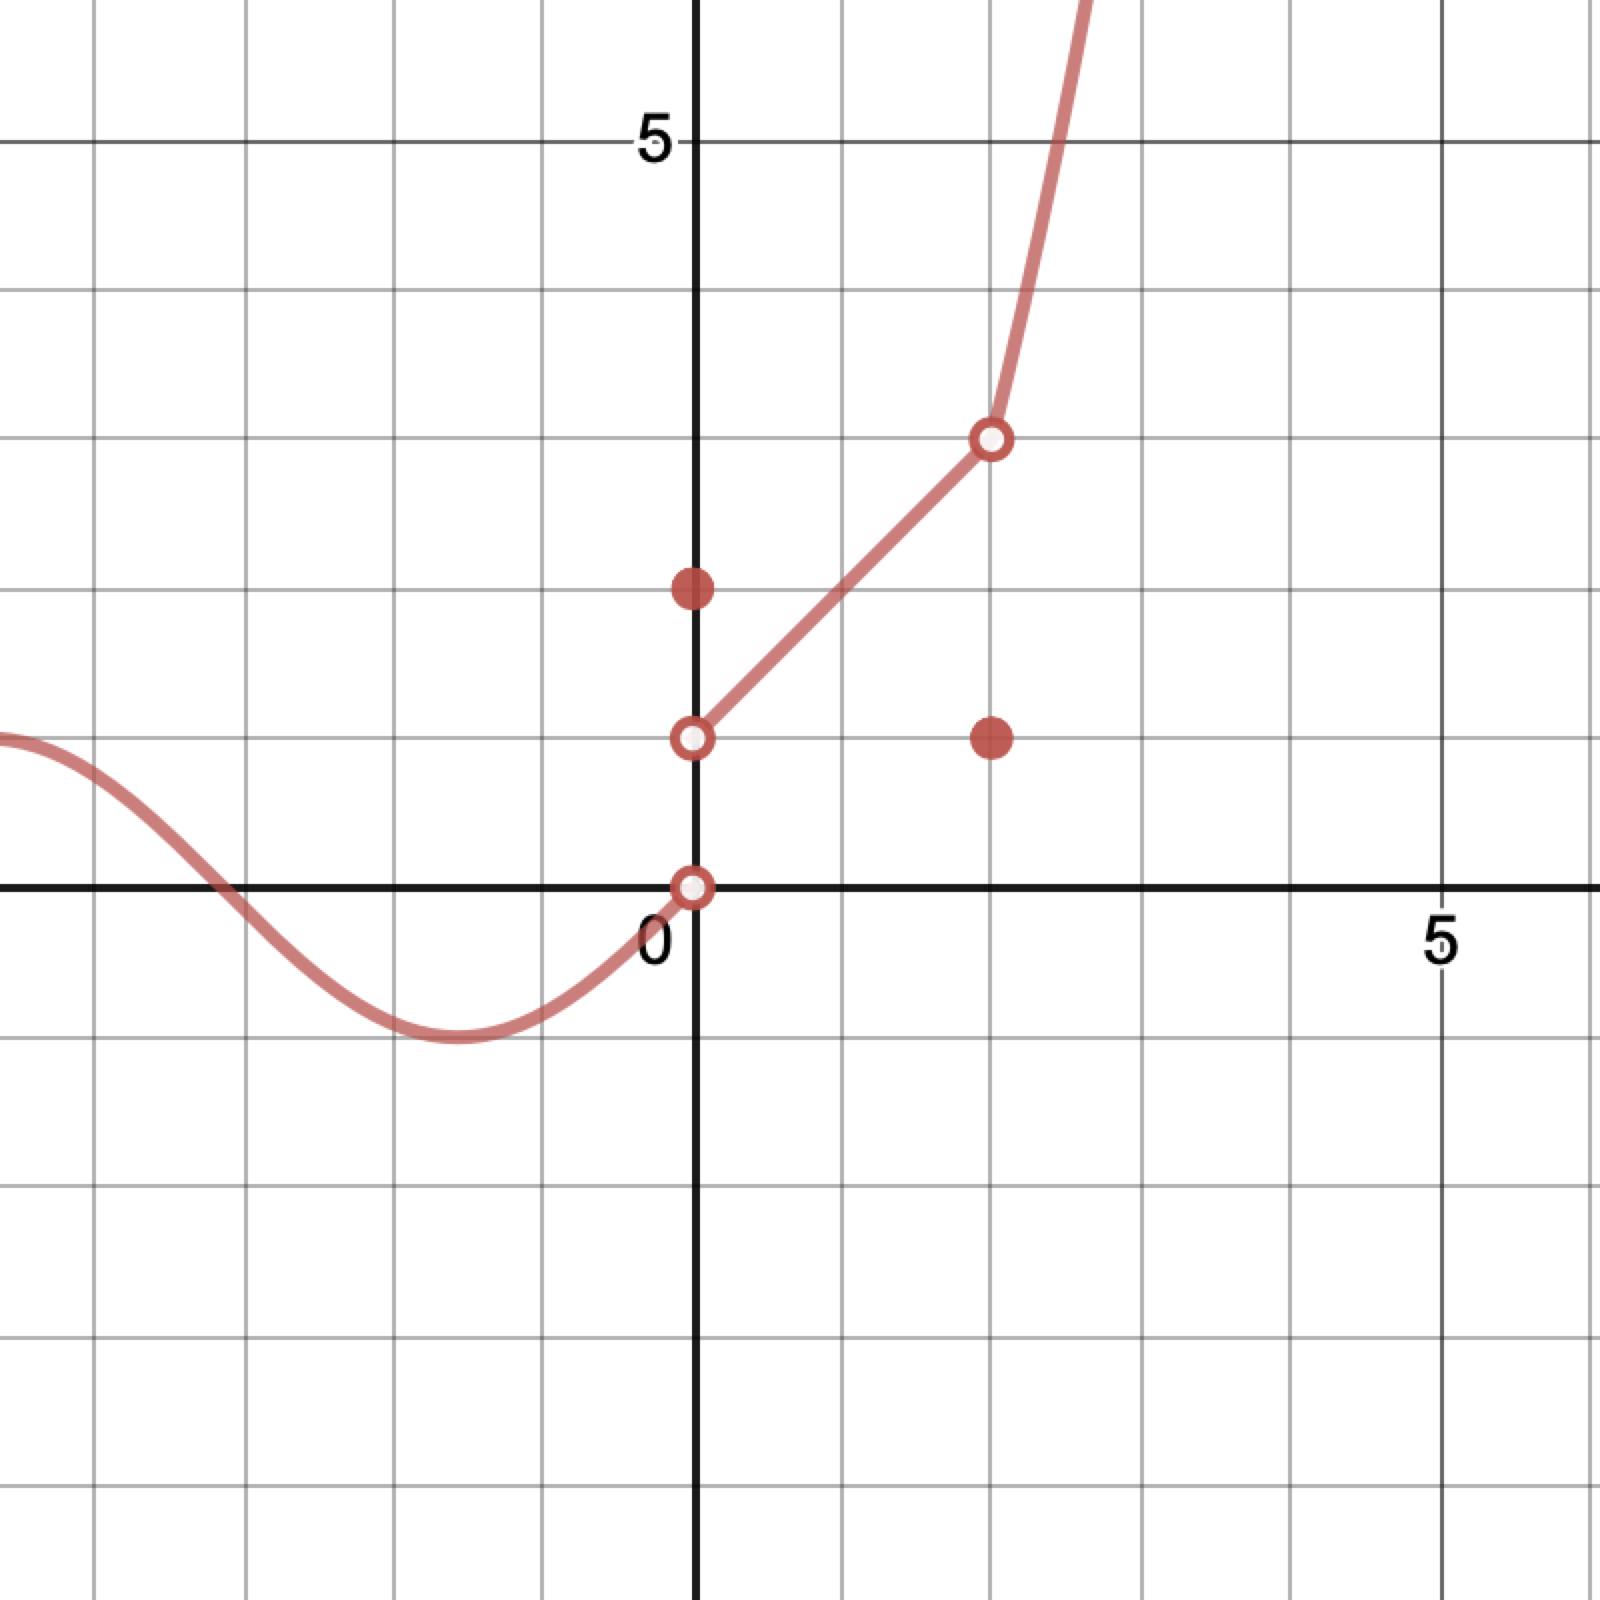
\includegraphics[width=\textwidth]{img/1_2_limit01.png}
\end{minipage}

}

\frame{
	\frametitle{Another approach}
	
	\begin{minipage}[t]{0.45\linewidth}
\rem{The function is $f(x) = \sin \frac{\pi}{x}$} 

\rem{$10^{-k}, 3\cdot 10^{-k}$}
\vspace{5in}
\end{minipage}
\hspace{0.5cm}
\begin{minipage}[b]{0.45\linewidth}
\centering
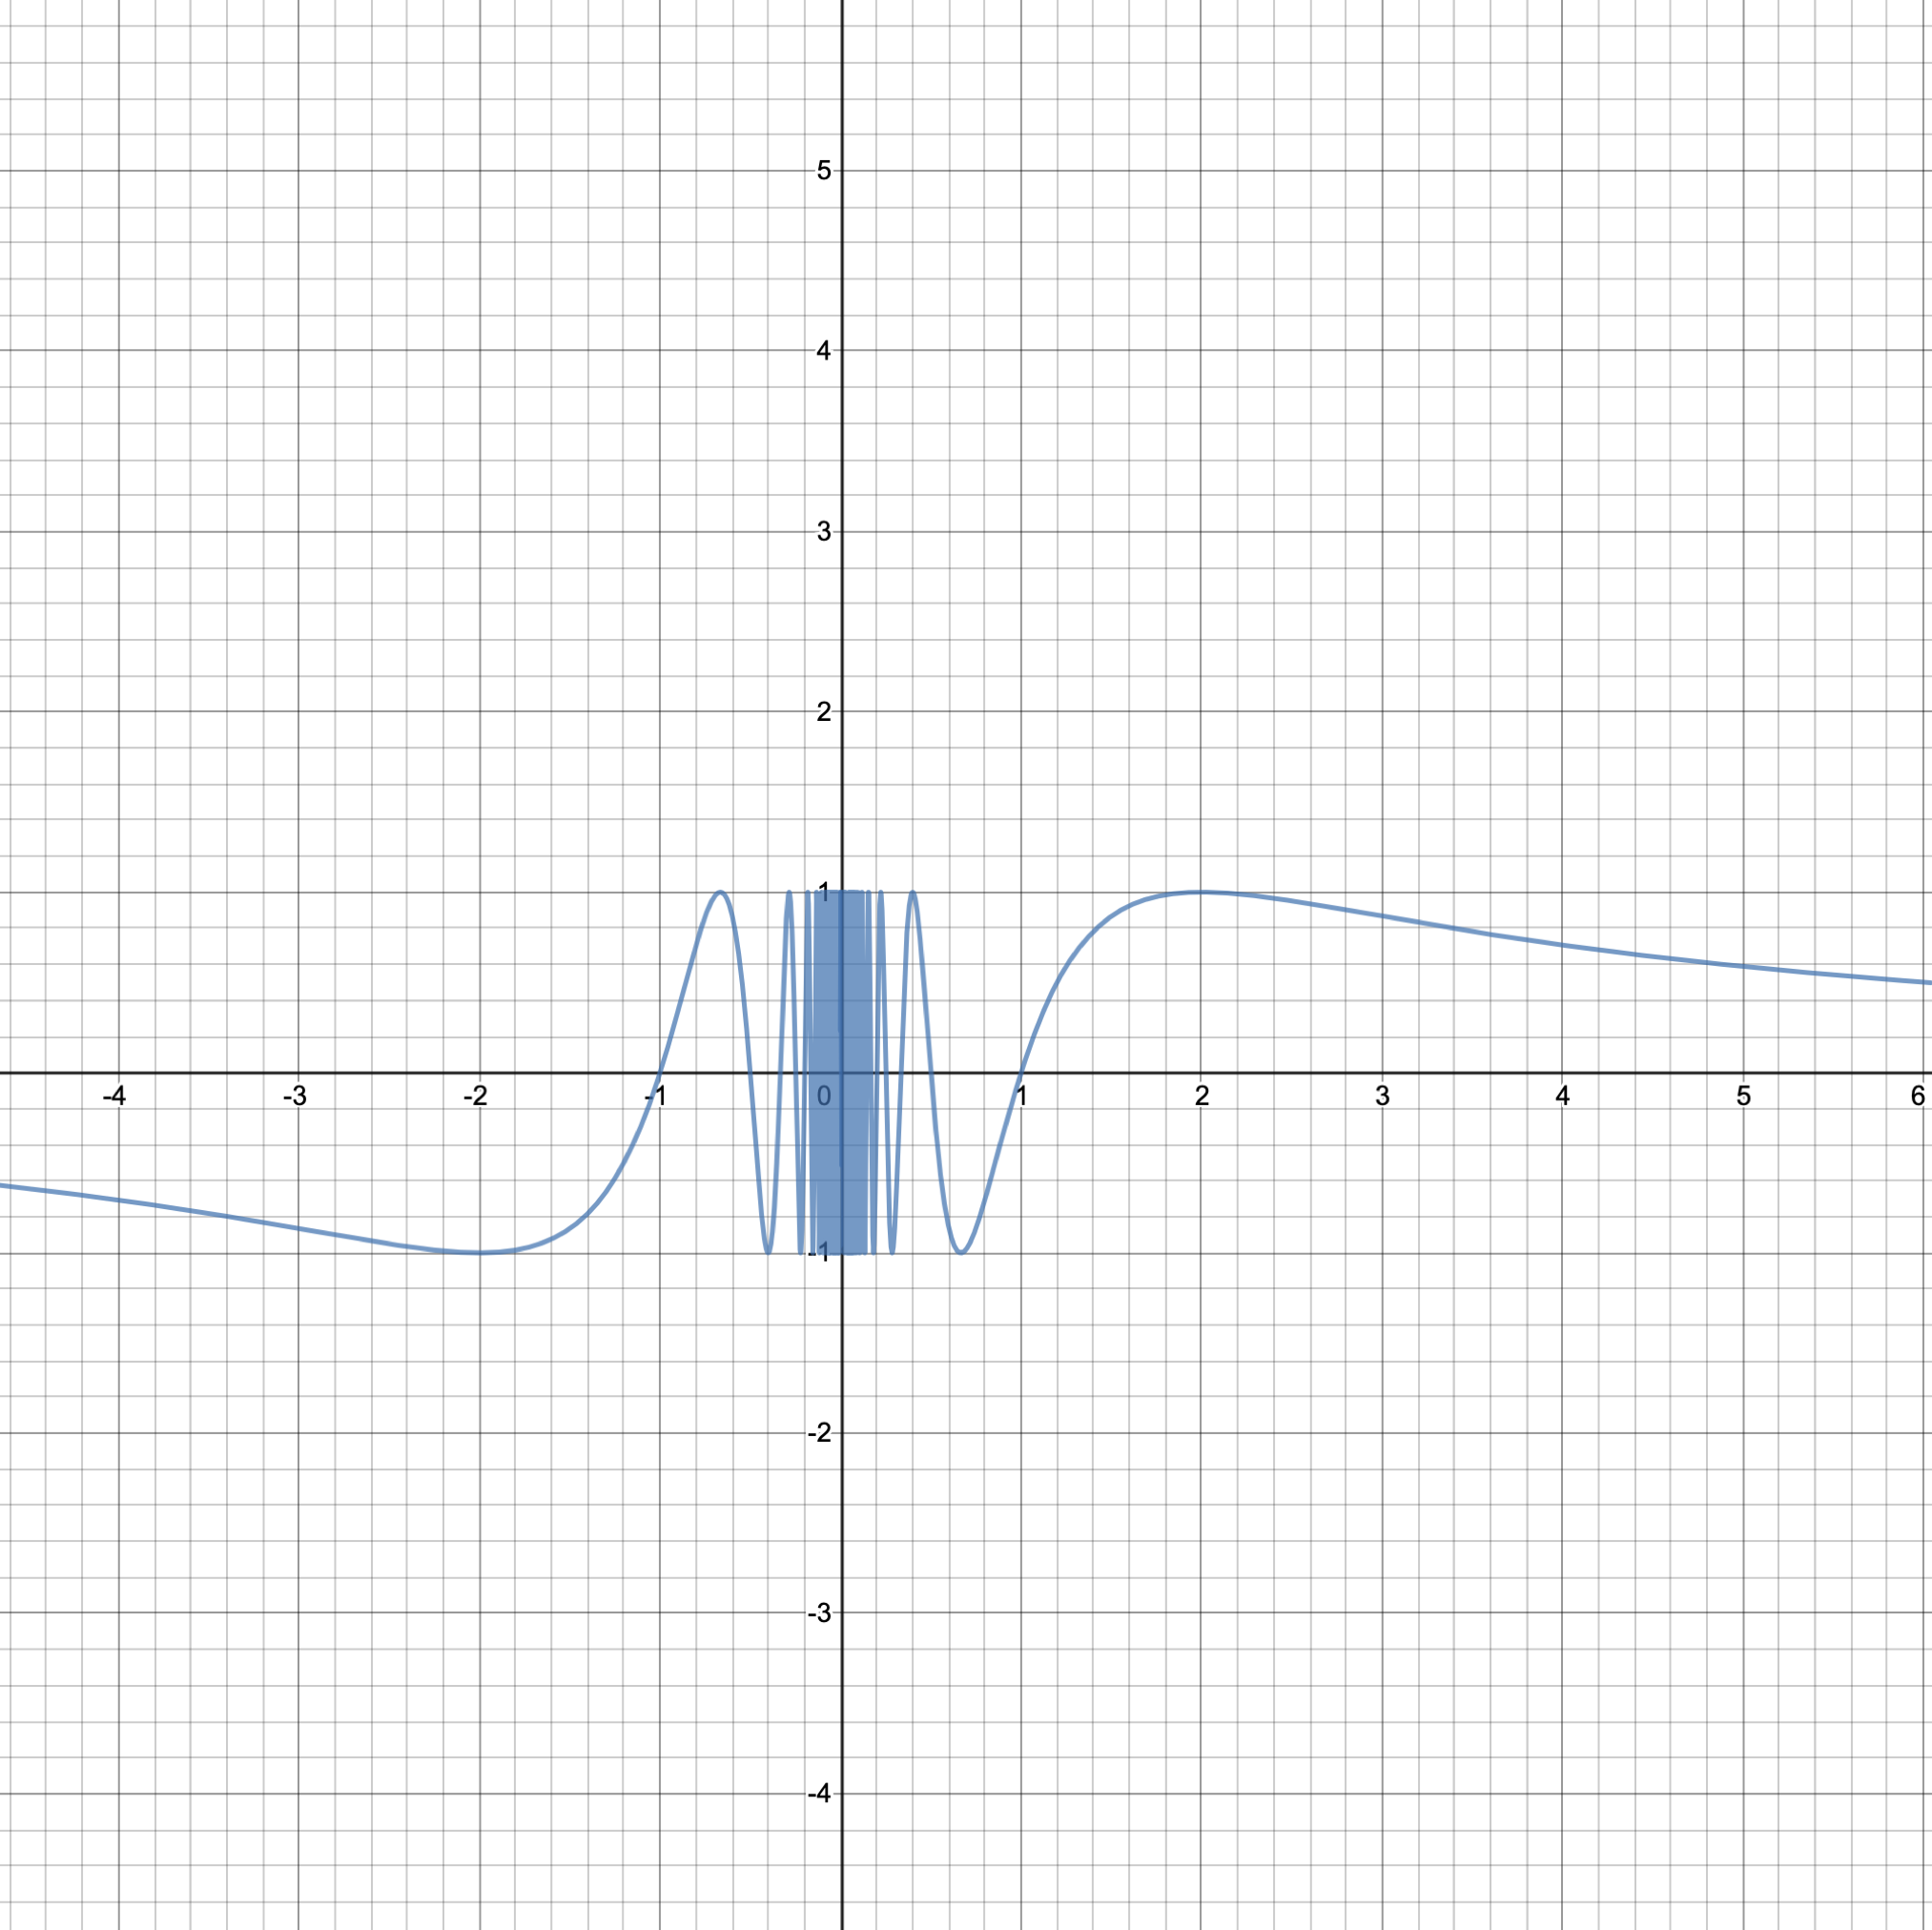
\includegraphics[width=\textwidth]{img/1_2_limit02.png}
\end{minipage}

}

\frame{
	\frametitle{Activity 1.2.2}

}

\frame{
	\frametitle{Instantaneous Velocity is the Limit of the Averages}
	
	\begin{itemize}
	\item That is: $IV_{t=a} = \lim\limits_{b\to a} AV_{[a,b]} = \lim\limits_{b\to a} \frac{s(b)- s(a)}{b-a}$\pause
	\item Equivalently: 
	\[
		IV_{t=a} = \lim\limits_{h\to 0} AV_{[a,a+h]} = \lim\limits_{h\to 0} \frac{s(a+h)-s(a)}{h}
	\]\pause
	\item Recall our discussion of the \textbf{\alert{Infinity Principle}}
\end{itemize}

}





\frame{
	\frametitle{Instantaneous Velocity is the Limit of the Averages}
	
	\begin{itemize}
	\item That is: $IV_{t=a} = \lim\limits_{b\to a} AV_{[a,b]} = \lim\limits_{b\to a} \frac{s(b)- s(a)}{b-a}$\pause
	\item Equivalently: 
	\[
		IV_{t=a} = \lim\limits_{h\to 0} AV_{[a,a+h]} = \lim\limits_{h\to 0} \frac{s(a+h)-s(a)}{h}
	\]\pause
	\item Recall our discussion of the \textbf{\alert{Infinity Principle}}
\end{itemize}

}

\frame{
	\frametitle{Activities 1.2.3--1.2.4}

}










\end{document}